%!TEX root = ../main.tex
\section{Introduction}
 node can be any kind of microcontroller, but this section will only address the case where a Zybo board is used. 
\mikkel{Something about this.}
\mikkel{Do we want to write here or in analysis why we use C and C++?}

\section{On-Vehicle Network}
%!TEX root = ../main.tex

\section{CAN bus}\label{sec:CANbus}
The CANOpen protocol runs on the CAN bus.
It was originally developed in the 1980's by Bosch.
It is a multi-master network, where each node connects to a common bus, and any node is then able to broadcast data to all other nodes.
The bus offers 1 Mbit/s on a bus up to 40 m of length. \todo{Martin: is this with or without the substantial overhead?}

\subsection{Physical Layer}\label{sub:CANphys}
The physical layer has three main parts: The CAN controller, the CAN transceiver and the bus itself. \\

The CAN controller can be implemented as a standalone IC, or in many cases integrated in the node itself.
The Zybo supports CAN, and an IP core is available, so the CAN controller is already given.\\

The CAN transceiver is connected to the controller by RX and TX voltage signals, and connects to the bus through two differential ports. 
The transceiver must support the standard ISO11898-2, as this is what the Sevcon motor driver uses.
The device SN65HVD232 from Texas instruments support this standard, and is supplied with 3.3 V, so it can be plugged right into the Zybo, and still communicate with the Sevcon even though its CAN bus uses $\si{5 \volt}$.
According to TI itself\cite{3.3V_CAN}, this family of $\si{3.3 \volt}$ transceivers are compatible and interoparable with other \si{5 \volt} transceivers, so long as they support the same standard.\\

The bus has to be made of twisted pair wires with a characteristic impedance of $\si{120 \ohm}$, and terminated at each end with a $\si{120 \ohm}$ resistor.
That means, that if the bus is broken at any point, no communication will work.
Alternately, it is possible to terminate each node, but this greatly reduces transmission speed, and will not be done.//

The transceivers have been mounted on boards, that plug directly into the Zybo's 12-pin PMOD connector, which will be stacked on top of each other. 
The schematic is shown below.

\begin{figure}[h!]
	\centering
	\includegraphics[width = 0.7\linewidth]{graphics/CAN_Schematic}
	\caption{Schematic of the two can transceivers. One board is build for two transceivers each with pads for termination}
	\label{fig:CAN_Schematic}
\end{figure}

The board has been designed to use the MIO ports, available in the PMOD JF. 
This is necessary to utilize the build in CAN controllers on the PS part of the Zybo.
Although the schematic contains two transceivers and two termination resistors, most of these devices are not mounted. 
Four boards will be made, all containing CAN0, C0 and the ZYBO connector. 
One board will also include the resistor R0 - this is the bottommost board
Another board will include R0, R1 CAN1, C1 and the SEVCON connector.
Ths is placed on top, to allow the SEVCON connector's screws to be accessible. 
The stack is visible below

\begin{figure}[H]
	\centering
	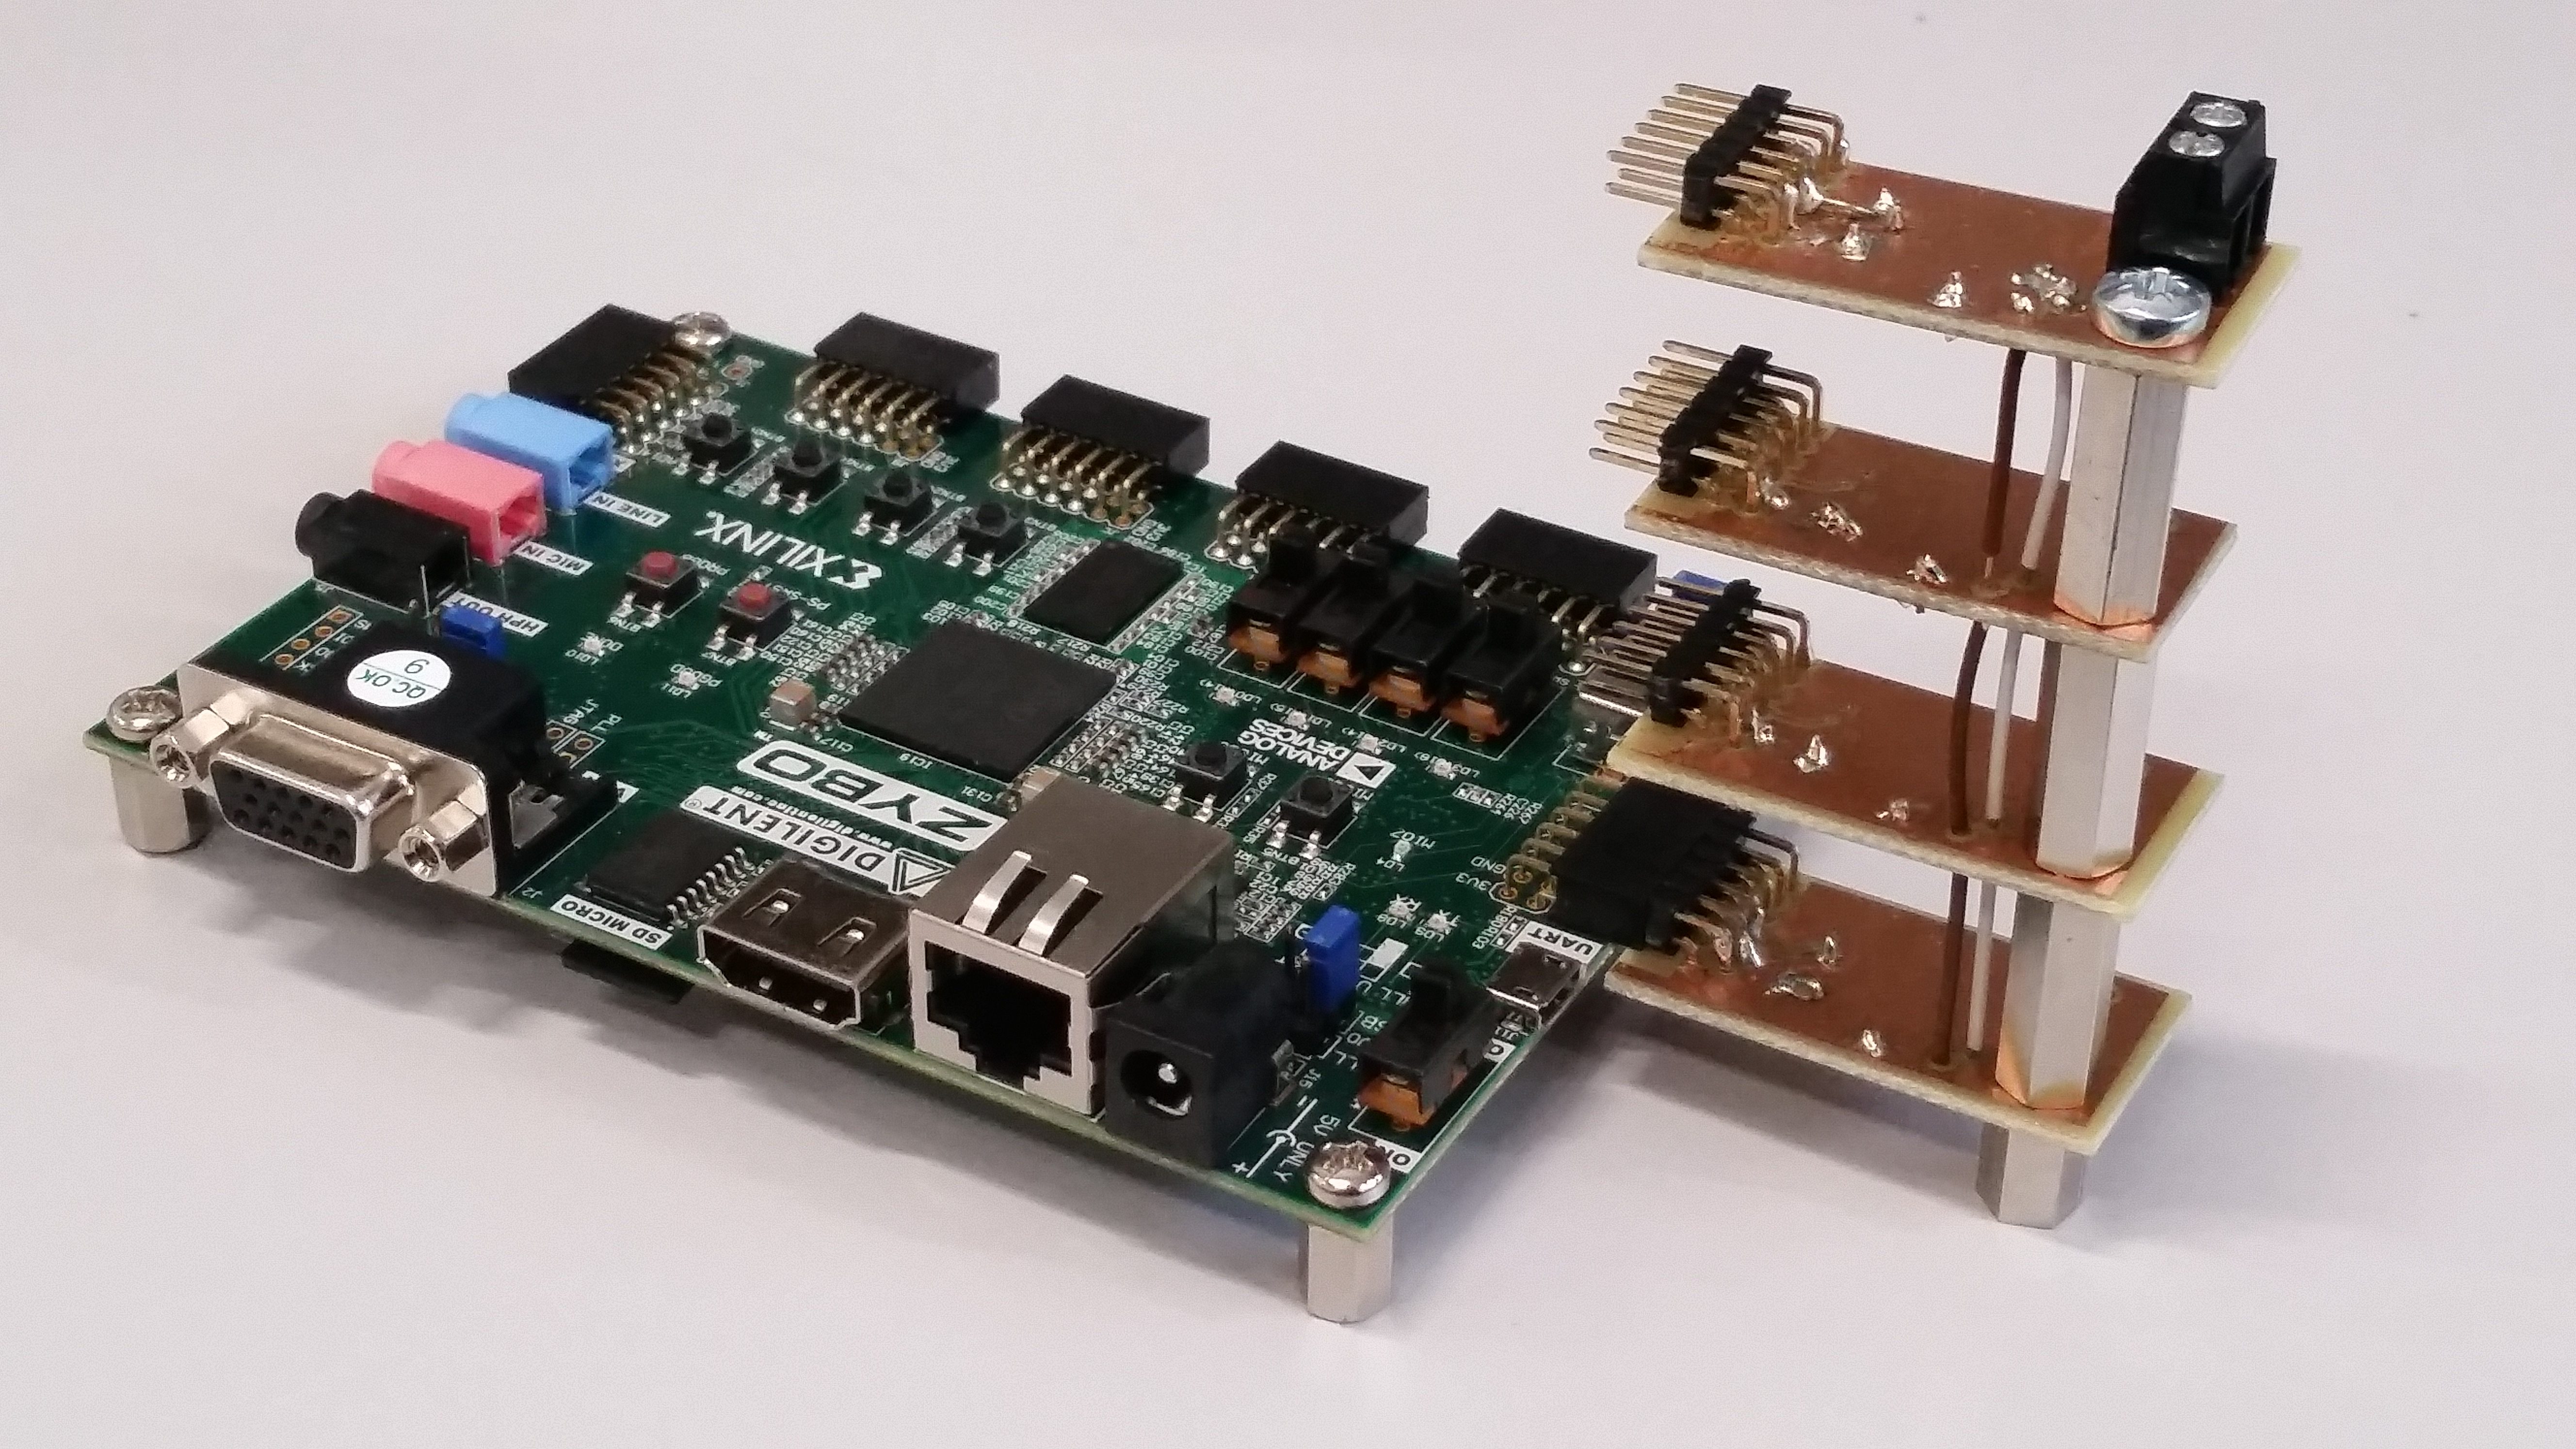
\includegraphics[width = 0.9\linewidth]{graphics/CAN_stack_picture}
	\caption{The CAN stack plugged into one Zybo}
	\label{fig:CAN_stack_picture}
\end{figure}

\subsection{Implementation of the Physical layer}\label{sub:CANphys_implementation}
The Zybo has two build in
\todo{I suppose you want to say built-in}

\subsection{Testing the CAN stack for a basic network}
After the design and printing of the stack board, testing it was the next step.
The test included using one the CAN controllers within the Zynq chip with the purpose of showing that a basic CAN network between two Zybo boards could be implemented using the stack.
Specifically, the one Zybo was sending the input value of the buttons to the network in order to be received by the second one and turn on the on-board LEDs as a result.
After designing a basic architecture in Vivado and writing a source code, the test was successful, thus proving the basic functionality of a CAN network.
All Zybo boards were programmed with the same architecture and source code.

\subsubsection{Architecture}
In order to realize the above test, enabling the CAN controller inside the Zynq chip as well as including two AXI GPIO cores were necessary. One AXI GPIO was setup as leds 4bits while the other one as btns 4bits as it can be seen in figure \ref{fig:CAN_Testing_Architecture}. 

\begin{figure}[h!]
	\centering
	\includegraphics[width = 0.9\linewidth]{graphics/Zybo_BasicTestingArchitecture_for_CAN}
	\caption{Block diagram featuring the testing architecture in Vivado.}
	\label{fig:CAN_Testing_Architecture}
\end{figure}

\subsubsection{Source Code}
%!TEX root = ../main.tex

\subsection{CAN protocol}\label{sub:CAN_protocol}
Due to the requirements of the on-kart network, it is decided to formulate a new protocol specifically for this project. The requirements are listed below.
\textbf{On-kart network requirements}:
\begin{itemize}
	\item Simple and easy to learn.
	\item Support for 16 nodes.
	\item Broadcast data.
	\item Defining message types.
	\item Variable data length - beyond 8 bytes per message
	\item Expandable.
	\item Commands: Start/stop broadcasting 
	\item Commands can be send to specific or all nodes
\end{itemize}

The basic CAN framework is retained for this protocol. 
The message ID is split in to two portions: The first four bits indicate the transmitting node ID, which will allow up to 16 nodes, all included. 
The last 7 bits of the message ID would contain an identifier for what the data portion of the frame contains.
Each node would then have a list of message IDs (11 bits), that it knows how to handle.
If a message is not on that list, the node will ignore it.
//
There are basically two types of nodes: The node containing with the Wifi link \todo[inline]{We should agree on names for the nodes, IE, Wifi node, IMU node and so on.}, and all other nodes.
Generally nodes can either produce data, and/or receive commands.
The Wifi node does neither produce any kind of data nor receive commands, but it odes receive data, and send out commands.
Therefore, there is a special case, for where the Wifi node is sending.
In this case, the subsequent four bits determines the recipient, leaving three bits for command type. 
For this part, command types are only "Start broadcasting" and "Stop broadcasting", but could be extended to for instance "Set parameter" or "Set value", where the data field will indicate which parameter, and what is's set to.



%!TEX root = ../main.tex
\subsection{Functions of the GoCAN Protocol}\label{sec:CAN_functions}
Some additional functionality is required in GoCAN to fulfill the requirements set.
This functionality is described throughout this section.

\subsubsection*{Timestamps}
As mentioned in section~\ref{sec:CAN-bus} the CAN protocol is not real time, therefore all data on the bus must be timestamped before transmission. 
The resolution of the timestamps has been decided to be 1 ms, as this leaves sufficient accuracy for the sensors analysed in this project.
This presents several challenges, in terms of what the time reference is and how to convey timestamps with adequate precision without creating too much overhead.
With internet access, the Epoch timestamp is available. 
This is infeasible in bare-metal code.
Instead a counter will be implemented on each node, incrementing an 32 bit integer every 1 ms.
This gives 49.6 days before overflowing.\\

Because a standard 32 bit integer takes 4 bytes, it would introduce a large overhead if the timestamp is sent with every message. 
Instead, each timestamp will determine the time of all subsequent data messages, until a new timestamp is sent. 
As an example, the pseudo code below describes the transmission of all nine axis of the IMU with the same timestamp.
Additionally, the IMU can transmit pressure and temperature measurements, but as these are slower signals, they would be transmitted at a lower rate.

\begin{lstlisting}
Send Timestamp
Send Ax, Ay, Az
Send Gx, Gy, Gz
Send Mx, My, Mz
Wait
Send Timestamp
Send Ax, Ay, Az
Send Gx, Gy, Gz
Send Mx, My, Mz
Send Pressure, Temperature
Wait
\end{lstlisting}

Lines 2-4 are measurements taken at the timestamp in line 1.
The WiFi node appends the corresponding timestamps to each of these nine data points with the corresponding timestamp.
Lines 7-10 refer to the timestamp at line 6.

\subsubsection*{Commands}
The WiFi node is capable of issuing commands on the network.
As described in section~\ref{sub:CAN_protocol}, it is possible to start and stop any specific or all other nodes from the WiFi node.

\subsubsection*{Synchronization}
Another specific command is the synchronization command. 
When the system starts all nodes will start polling their Rx FIFO for this sync command. 
When this command is received, the node will start the millisecond timer.

\subsubsection*{Multiframe Messages}
Due to the limited data length of a CAN frame, it is likely necessary to support multiple frames per message. 
Generally it is better to use all 8 bytes of data in one frame, to reduce the relative size of the overhead, and in case a dataset isn't easily split into 8 byte portions, it might be easier to bundle it all together and send as multiple full frames. 
In the message ID of all but the first frame of a multi-frame message the \texttt{new message}, to make it highest priority.
That way a message will not be interrupted by other messages from other nodes.
The construction and interpretation of these multiframe messages are described in sections~\ref{sec:sensor_node} and~\ref{sec:frontend}.

\subsubsection*{Datatype and Scaling}
As most sensor data comes from sources of limited resolution, the optimal solution would be to send only the number of bits that are measured. 
In some cases however that is not possible, and a better solution is to round up or down to the nearest byte, and send the data as a fixed point data type.
Intead of defining a new datatype, an integer of appropriate length will be used instead, and the object dictionary will define the scaling. \\

As an example, the message described in table~\ref{tab:message17_OD} contains four data points of 2 bytes. 
This contains the current measurements on the three phases along with the electrical position of the rotor.
An example is described in table~\ref{tab:message17_OD}.

\begin{table}
	\centering
	\begin{tabular}{l|l|l|l|l|l}
		Message ID & DLC & $\mathrm{I_a}$ & $\mathrm{I_b}$ & $\mathrm{I_c}$ & $\mathrm{\Omega _e}$ \\ 
		\hline
		10100001001 & 1000 & 414 & -1545 & 1131 & 13090 \\
		\hline
		 & & 25.9 A & -96.6 A & 70.7 A & 1.31 rad
	\end{tabular}
	\caption{Example of message data from line 17 of table~\ref{tab:OD}}
	\label{tab:message17_OD}
\end{table}
According to table~\ref{tab:OD}, there are two scaling factors defined, one for currents and one for angle. 
The bottom line of table~\ref{tab:message17_OD} shows the resolved measurements.

%!TEX root = ../main.tex
\subsection{Implementing CAN utilizing XCanPs}\label{sec:methods_to_implement_can}

\mikkel{DONE:move axi can to analysis.}
\mikkel{move assymetric multiprocesssing to future work}
\mikkel{ move bare metal first}
\mikkel{split from linux part.}
\martin{The can controllers do not have anything to do with xilinux. Does Xilinux provide drivers for the can controllers on the zynq? CAN controllers vs CAN drivers Issue - Some things rephrased.}

This section includes the process that was followed to enable the CAN controller in Linux.
The purpose of this was to gain access to the controllers from Linux.
Using this operating system was necessary for using the required USB interfaces, logging the data into files as well as utilizing the network tools to establish an ad-hoc network.
The steps for this were to modify certain files related to the kernel configurations and the device tree settings.

\subsubsection*{Enabling the CAN Controller Drivers}

According to Xilinx documentation, the process for enabling the CAN controllers on the Zynq7 Processing System, the Linux CAN driver guide \cite{Xilinx_wiki_Linux_CAN_driver} was needed to be followed.
Specifically, the Kconfig file under the path \ref{code:can_kconfig_pathfile} needed to be configured.
The entry at line 128 was changed as seen in code \ref{code:can_kconfig_contents_line128}.
Originally, lines 130 and 131 were as seen in code \ref{code:can_kconfig_original_line130}.

\begin{lstlisting}[caption={CAN Kconfig pathfile.},numbers=none,label=code:can_kconfig_pathfile]
/usr/src/kernels/3.12.0-xillinux-1.3/drivers/net/can
\end{lstlisting}

\begin{lstlisting}[firstnumber=128,caption={Kconfig file contents from line 128.},label={code:can_kconfig_contents_line128}]
config CAN_XILINXCAN
	tristate "Xilinx(*@ @*)CAN"
	depends on NET [=y] && CAN_DEV [=y] && CAN [=y] && 
        (ARCH_ZYNQ || MICROBLAZE [=y])
	default y
\end{lstlisting}

\begin{lstlisting}[firstnumber=130,caption={Original content of lines 130 and 131.},label={code:can_kconfig_original_line130}]
	depends on CAN && (ARCH_ZYNQ || MICROBLAZE)
	default n
\end{lstlisting}

The next step of the process was the modification of the device tree settings file, requiring an entry for the CAN PS to be inserted.
The necessary file was located under the boot folder named as seen in \ref{code:dts_file_zybo}.
The modifications can be seen in code \ref{code:dts_changes_zybo} for can controllers as well as for the AXI CAN core.

\begin{lstlisting}[numbers=none,caption={Device tree settings file and its path.},label={code:dts_file_zybo}]
/boot/xillinux-1.3-zybo.dts
\end{lstlisting}
\catalin{Double quotes are problem here as well. FIX THEM WHENEVER}
\begin{lstlisting}[caption={Device tree settings changes.},label={code:dts_changes_zybo}]
zynq_can_0: can@e0008000 {
        compatible = xlnx,zynq-can-1.0;
        clocks = <&clkc 19>, <&clkc 36>;
        clock-names = can_clk, pclk;
        reg = <0xe0008000 0x1000>;
        interrupts = <0 28 4>;
        interrupt-parent = <&intc>;
        tx-fifo-depth = <0x40>;
        rx-fifo-depth = <0x40>;
    };
axi_can_0: axi-can@40000000 {
        compatible = xlnx,axi-can-1.00.a;
        clocks = <&clkc 0>, <&clkc 1>;
        clock-names = can_clk,s_axi_aclk;
        reg = <0x40000000 0x10000>;
        interrupt-parent = <&intc>;
        interrupts = <0 59 1>;
        tx-fifo-depth = <0x40>;
        rx-fifo-depth = <0x40>;
        };
\end{lstlisting}

Unfortunately, the above steps did not enable the drivers successfully.
After the changes, the CAN devices were still not visible in Linux and thus, connection to the CAN network was not feasible.
Research was done by the authors in why this could not be accomplished.
It was found that there were some naming inconsistencies between the guide and the Device Tree Settings file present in Linux running on the Zybo. Specifically, all the devices' names in the file are prepended with ps7.
A new set of changes with this naming convention was done, but with no success.\\

The files mentioned above were modified in the Linux running on the Zybo.
It was expected the changes to take effect after rebooting the system, which was not the case.
Another approach to this, was to build a new kernel containing these changes and to entirely build a new Linux system for the Zybo.
This proved to be unachievable because of the various patches that had been applied to the initial kernel by Diligent Inc. and Xilinx.
A new updated kernel with those patches could not be built MIKKEL.
\mikkel{say a few words why could not be built, just the main reason, after ...could not be built ....}

%The architecture can be seen in figure \ref{fig:CAN_Arch_with_AXI_CAN}.

%\begin{figure}[h!]
%	\centering
%	\includegraphics[width = 1.2\linewidth]{graphics/Zybo_Arch_with_AXI_CAN.png}
%	\caption{Block diagram featuring the architecture in Vivado with the AXI CAN core.}
%	\label{fig:CAN_Arch_with_AXI_CAN}
%\end{figure}


\catalin{Explain the code in more detail. Also mention the interrupt part for gpio.}
\subsection{CAN Controller Software}
\subsubsection{Implementation in code}~\\
As mentioned in section \ref{sub:Basic_SourceCode}, the code was based on the xcanps polled example available by Xilinx documentation.
The important functionalities that needed to be provided by the final software version included:
\begin{itemize}
\item receiving and sending of frames
\item creating the message id
\item decoding of the message id parts, such as the node id, the message type etc. \catalin{what else?}
\item handling button interrupts
\item controlling the LEDs
\item accepting and ignoring messages according to the subscriptions list
\end{itemize}
\catalin{What other functionalities? And, 1st letters capitals or not?}
The figure \ref{fig:SeqDiagram_SendFrame} shows the procedure of sending a frame to the CAN network containing data, which makes use of the protocol function createMsgID().
After returning the message id, the id and the data are put into the TxFrame to be sent once the FIFO has space.
The actual sending is done with a call to the XCanPs function XCanPs\_Send().
\\
Similarly, the procedure of receiving a frame is shown in the figure \ref{fig:SeqDiagram_RecvFrame}.
The node once it calls the RecvFrame() function, it waits in a loop until it receives a frame. Then, it checks the subscriptions in order to forward the packet for further processing or to ignore it.


This was achieved by implementing a set of functions and an array variable of subscriptions for each node.

\begin{figure}[h!]
	\centering
	\includegraphics[width = 1.1\linewidth]{graphics/SeqDiagram_SendFrame.pdf}
	\caption{The sequence diagram of the process of sending a frame.}
	\label{fig:SeqDiagram_SendFrame}
\end{figure}

\begin{figure}[h!]
	\centering
	\includegraphics[width = 1.1\linewidth]{graphics/SeqDiagram_RecvFrame.pdf}
	\caption{The sequence diagram of the process of receiving a frame.}
	\label{fig:SeqDiagram_RecvFrame}
\end{figure}

\begin{figure}[h!]
	\centering
	\includegraphics[width = 1.1\linewidth]{graphics/StateDiagram_CanStackTestCode.pdf}
	\caption{Behavioral diagram of the basic source code.}
	\label{fig:CAN_Testing_StateDiagr_Code}
\end{figure}
%!TEX root = ../main.tex
\subsection{Object Dictionary}\label{sub:OD}
In order to ensure that all message IDs are unique, an Object Dictionary is declared for this high level protocol.
The name is inspired from CANopen, but unlike the CANopen Object Dictionary, this refers to the messages being transmitted on the, and not the parameters or variables on the CANopen node.
Because of this, some variables appear in several message IDs, as it might be desirable to reconfigure some nodes to send different data, and the node should group data together to reduce the number of frames.\\

At this time, there are four nodes in the Object Dictionary with their node ID in hex: Wifi 0x1, IMU 0x3, Sevcon 0x7 and GPS 0xD.
The Wifi node is considered the master, and can command the other nodes, and as such it's portion of the OD is a bit different. 
Common for the other three nodes is that the message type 0x01 is a four byte timestamp.
Other than that, data messages start from 0x08.\\

Table~\ref{tab:OD} in appendix~\ref{app:OD} on page~\pageref{tab} contains the Object Dictionary in its current form.


\section{Off-Vehicle Network}
\label{sec:wifi}
%!TEX root = ../main.tex
\section{Networking}
The system deviced throughout this report seeks to ease the task of collecting data from the go-kart.
This is done by creating a network on the go-kart which allows the user to more easily add additional sensors.
In addition to providing a flexible platform for adding sensors, it will collect the data produced by the sensors on the network.
A goal with the project is to be able to monitor relevant data live through some interface.
To properly monitor data collected during driving it is necessary to maintain a live feed from the go-kart to the observer.
\\~\\
As mentioned above, there are two major functions to the system; recording of data and monitoring of data.
The recording is done on the go-kart using embedded hardware, specifically the Zybo platform is used to interface to the sensors.
The monitoring is done using a PC.
Monitoring is less time critical than the recording as it is simply meant for human readability.
For this reason, and to ease the workload, it has been decided to use a wifi connection between the go-kart and the PC.
Wifi, or even TCP/IP over ethernet is not viable on the go-kart between the Zybo boards due to the potentially long lag in that protocol.
A different network type will have to be devised for the embedded portion of the system.
This splits the network up into two parts, one that links the PC to the go-kart and one that links each component on the go-kart.
See figure \ref{fig:basic_network}.

\begin{figure}
	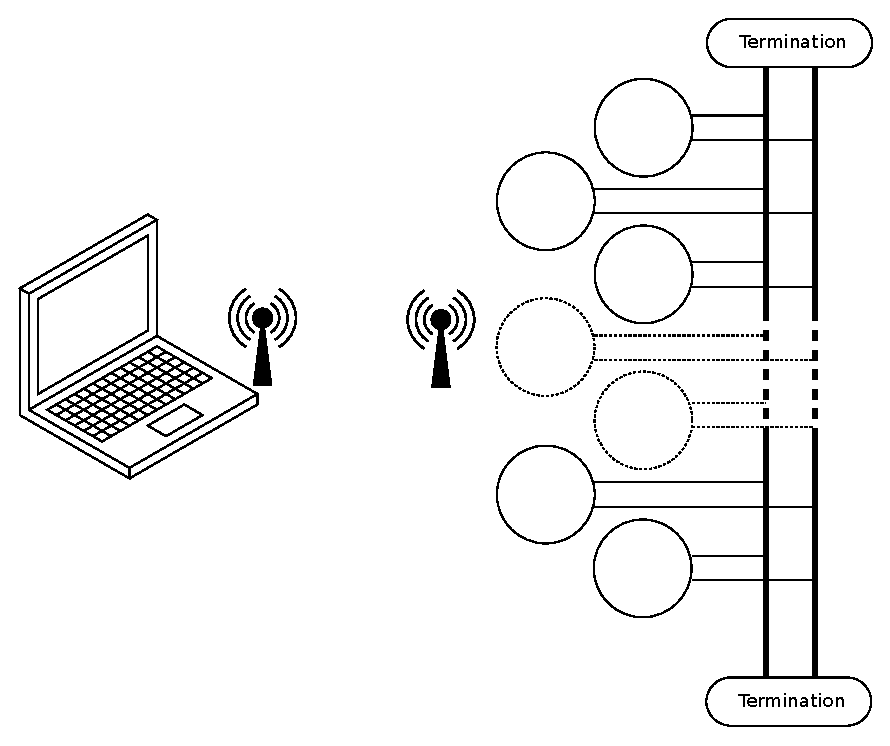
\includegraphics[width=.75\linewidth]{graphics/basic_network}
	\caption{A line of text}
	\label{fig:basic_network}
\end{figure}

These will be referred to as the off-kart network and the on-kart network, respectively, throughout the remainder of the report.
The following sections will explore the creation of both of these networks in turn.

\subsection{Off-Kart Network}
As mentioned above, the off-kart network is done using wifi.
It was chosen to use this method as all modern laptops are equipped with the capability of connecting to such a network.
Hereafter the challenge lies in establishing an ad-hoc network between a zybo board and a PC.
This network is created using the a USB-Wifi dongle on the Zybo board. 
The following script is run to bring down the device, change the network type to ad-hoc, bring up the device, create the ad-hoc network and, finally, assign an IP-address to the device.
\begin{lstlisting}
sudo ip link set wlan0 down
sudo iw wlan0 set type ibss
sudo ip link set wlan0 up
sudo iw wlan0 ibss join go-kart 2412
sudo ifconfig wlan0 192.168.10.9
\end{lstlisting}
It is verified working using the ping command from both the Zybo board and to the PC and vice versa.
Below is a thorough description of the challenges encountered while setting up this device as well as a brief explanation of the choice of device.
\\~\\
Two methods were immediately available for use: A usb wifi dongle and a PMOD wifi interface.
As the name implies, the latter is designed to be compatible with the PMOD interfaces on the zybo board (and a range of similar boards offered by Digilent Inc.).
It converts TCP/IP to SPI and vice versa.
However, since the zybo boards are already running a linux distribution, it was decided to attempt connecting through the usb wifi dongle.
This decision marked the beginning of a long journey, the highlights of which are discussed below. 
\\~\\
The first step was to ensure that the correct drivers are present on the system.
The usb dongle is a TP-LINK TL-WN722N.
This device uses the Atheros AR9271 chipset and is on the list of supported devices for the ath9k\_htc driver on wireless.wiki.kernel.org.
Running \texttt{dmesg} prints the kernel log, revealing, amongst other things, what drivers are loaded.
\begin{lstlisting}
dmesg | grep ath
[10.329564] usb 1-1: ath9k_htc: Firmware htc_9271.fw requested
[10.332438] usbcore: registered new interface driver ath9k_htc
\end{lstlisting}
Additionally:
\begin{lstlisting}
lsusb | grep Ath
Bus 001 Device 002: ID 0cf3:9271 Atheros Communications, 
	Inc. AR9271 802.11n
\end{lstlisting}
As per these commands the operating system (OS) has correctly detected and loaded the driver.
The \texttt{iproute2} package contains the utilities used to manipulate TCP/IP connections.
\begin{lstlisting}
ip link show
1: lo: <LOOPBACK,UP,LOWER_UP> mtu 65536 qdisc noqueue 
	state UNKNOWN mode DEFAULT group default 
    link/loopback 00:00:00:00:00:00 brd 00:00:00:00:00:00
2: eth0: <BROADCAST,MULTICAST,UP,LOWER_UP> mtu 1500 qdisc pfifo_fast 
	state UP mode DEFAULT group default qlen 1000
    link/ether 00:0a:35:00:01:22 brd ff:ff:ff:ff:ff:ff
3: wlan0: <BROADCAST,MULTICAST> mtu 1500 qdisc mq 
	state DOWN mode DEFAULT group default qlen 1000
    link/ether ec:08:6b:1b:41:b3 brd ff:ff:ff:ff:ff:ff
\end{lstlisting}
The device has been given the identifier \texttt{wlan0}.
It can be brought up by:
\begin{lstlisting}
ip link set wlan0 up
ip link show wlan0
3: wlan0: <NO-CARRIER,BROADCAST,MULTICAST,UP> mtu 1500 qdisc mq 
	state DOWN mode DEFAULT group default qlen 1000
    link/ether ec:08:6b:1b:41:b3 brd ff:ff:ff:ff:ff:ff
\end{lstlisting}
At this point the device is up, as can be seen on the list of flags:
\begin{lstlisting}
<NO-CARRIER,BROADCAST,MULTICAST,UP>
\end{lstlisting}
However, the \texttt{NO-CARRIER} flag is also set.
This flag indicates a fault on the physical layer, i.e. a disconnected network cable or similar.
In an attempt to isolate the error the dongle was connected to a PC.
The dongle worked flawlessly on the PC and connected to the internet after bringing down the standard interface.
Clearly, there are differences between the two systems, one or more of which were causing the 
Eliminating these differences 
\subsection{On-Kart Network}

\section{Nodes}
%!TEX root = ../main.tex
\mikkel{An introductiontion needs to be here!}
The designed network generally have two types of nodes, a generic sensor node and the wifi node.
This section will seek to design and implement software that adheres to the requirements listed earlier.
A node can be any kind of microcontroller, but this section will only address the case where a Zybo board is used. 

\subsection{Sensor Node}
\label{sec:sensor_node}
The requirements state that it should be simple to add new sensor nodes to the system. 
To realize this the node software should be designed to be modular.
It should be easily identified what software and what interface a developer of a new sensor node must adhere to.

An example of a node can be seen in figure \ref{fig:gps_node}.

\mikkel{Where to put this text?}

%The coming sections will explain the design of the node software that will provide the mentioned functionality using the design requirement.

\begin{figure}[!h]
\centering
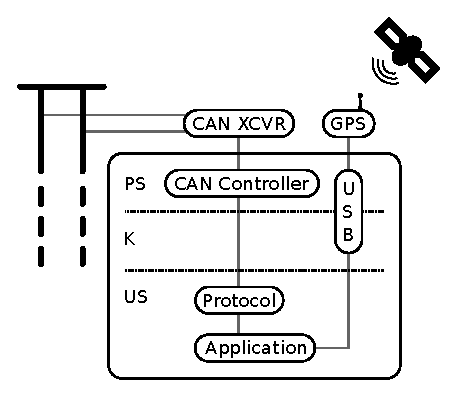
\includegraphics[width=0.5\textwidth]{graphics/analysis_gps.eps}
\caption{GPS node implemented on Zybo board.}
\label{fig:gps_node}
\end{figure}
\mikkel{Maybe change this figure to reflect the real system???}

This specific node has a GPS attached to it connected through a USB interface, but in general it could be any kind of data producing unit connected through any kind of interface.
\mikkel{How do we do this referencing nicely?}
From the requirements, table \ref{tab:requirements}, it is found that the sensor node software needs to fulfill requirements 1,2,6,10,11,12,20 and 21.
From the analysis section is it clear that a sensor node has the following responsibilities:

\begin{itemize}
\item Get data from associated sensor.
\item Pack data according to the specified protocol.
\item Construct CAN package
\item Send data using a CAN controller.
\item Get data from CAN network.
\item React to commands sent to it.
\end{itemize}

As described earlier the responsibility of sending data using a CAN controller and receiving data from the CAN network is done in the earlier described bare-metal code.
This section will focus on the designing and implementing code that provide the rest of the listed functionalities.

Analyzing on the procedure when data goes from a sensor to the CAN program resulted in the block diagram of figure \ref{fig:block_gps}.

\begin{figure}[!h]
    \centering
    \begin{subfigure}[b]{0.33\textwidth}
        \includegraphics[width=\textwidth]{graphics/FlowChart_Node_Packing}
        \caption{Ingoing data....}
        \label{fig:filter_full}
    \end{subfigure}
    ~
    \begin{subfigure}[b]{0.33\textwidth}
        \includegraphics[width=\textwidth]{graphics/FlowChart_Node_Unpacking}
        \caption{Two minu.}
        \label{fig:filter_2}
    \end{subfigure}
        \caption{Outgoing data.}
           \label{fig:filter_fulll}
\end{figure}
To design modular software it needs to be analyzed which blocks are the same for all nodes and which are sensor specific.
The sensor specific tasks are found to be extracting data from sensor and to pack data according to the protocol.
The remaining tasks are the same for all sensor nodes in the system. 
The procedure when data is going from the CAN program to the node is shown in figure \ref{fig:block_gps}.
All tasks are found to be generic for all sensor nodes.

\subsubsection*{Class diagram}
Based on the previous analysis a class diagram was developed and can be seen in figure \ref{fig:node_class_diagram}.
Classes to the right of the dashed horizontal is sensor specific and should be developed for each specific sensor.
Classes to the left are agnostic to all data they receive going from the sensor and to the CAN network.
They are generic classes and should be reused when developing new nodes.

\begin{figure}[!h]
\centering
\missingfigure[figwidth=1\textwidth]{Class diagram}
\caption{Class diagram showing node software.}
\label{fig:node_class_diagram}
\end{figure}

A struct containing all fields of a data packet in boolean data types is defined in listing \ref{code:data_packet}.  

\begin{lstlisting}[caption=Struct for data packet.,label=code:data_packet]
struct data_packet {
  std::bitset<1> sof;
  std::bitset<4> node_id;
  std::bitset<4> n_data_bytes;
  std::bitset<6> messagetype;
  std::vector<bool> data;
(*@\makebox[\linewidth][c]{$\smash{\vdots}$}@*)
};
\end{lstlisting}
It will be passed between the classes and they will each add their own information. 

The classes and their tasks from figure \ref{code:data_packet} will be explained here.

\mikkel{Put color explanation here?}

~\\ \par \textbf{GPS class} ~ \\
The GPS class needs to extract data from a connected GPS unit and update its own variables with that data.
The specific GPS unit used in this project has a USB interface and uses the NMEA protocol to format data.

~\\ \par \textbf{Packer\_GPS class} ~ \\
The Packer\_GPS class is also sensor specific and is the link between the sensor and the data agnostic node.
It is hard-coded with the message types that the sensor is allowed to send onto the network.
It has the responsibility to pack data according to the developed protocol.
Data in the form of a vector of booleans are then put into the \texttt{data\_packet} struct and passed to the node class.
The reason for making a separate class for the packer and not putting the functionality into the GPS class is that if the specification of the protocol or message types change, only this class needs to be modified.

~\\ \par \textbf{Node class} ~ \\
The Node class gets \texttt{data\_packets} from the Packer class it then needs to append its node id to it.
It needs to create a timestamp \texttt{data\_packet} each time data is to be sent.
In order to create the time message the class needs to keep track of milliseconds since last received synchronize message.
The class receives start, stop or synchronize events from the protocol class and reacts to those accordingly.

~\\ \par \textbf{Protocol class} ~ \\
The protocol class receives \texttt{data\_packets} from the node class. 
If it receives \texttt{data\_packets} where there are more than eight data bytes it needs to create additional \texttt{data\_packets} and distribute data to them. 
The additional \texttt{data\_packets} must have the same node id and message types, but the start of frame, sof, bit should be set accordingly.
The class also needs to append number of data bytes, \texttt{n\_data\_bytes}, to each \texttt{data\_packet}.
On \texttt{data\_packets} coming from the CAN network the class needs to use the last two bits of the messagetype to decode which command is sent to the node.
\martin{This may or may not be adressed to the node, so it should be handled in node.}

~\\ \par \textbf{CAN\_link class} ~ \\
The CAN\_link class has the responsibility of transferring and receiving data to and from the CAN program.
As this interface has not yet been implemented this class makes use of the standard input and output. 
Meaning that data from the sensor will be printed in the shell and data to the node should be written to the shell. 

\subsubsection*{Passing data between classes}
Communication between classes is realised by using the producer-consumer pattern.
As the name implies one class produces data and puts this in a queue where another class consumes by taking data out of the queue.
To get the producer and consumer functions to run in parallel they are run in separate threads.
All queues are protected by a mutex to make the software thread-safe.

\subsubsection*{Node class functionality}
The functionalities of the Node class on outgoing data is implemented using a state machine.
It is shown in figure \ref{fig:state_machine}.
\begin{figure}[!h]
\centering
\includegraphics[width=1\textwidth]{graphics/StateDiagram_Node.pdf}
\caption{State machine.....}
\label{fig:state_machine}
\end{figure}
When the variable \texttt{run} is equal to 1, the node should output sensor data.
\texttt{run} is being updated by the thread that handles incoming commands.
It will then go the clear state and clear all variables and wait for data. 
When data is present it will move through the states create time packet, get data and send data. 
If at any point \texttt{run} is set to 0 the state machine will go to the stop state.


\subsubsection*{Implementing a new Sensor node}
When developing a new node with another sensor the generic classes CAN\_link, Protocol and Node should be used. 
New classes should be developed to extract data from sensor, pack data according to protocol and put the data in a data\_packet.
It is advantageous to implement this functionality into Packer\_Sensor and Sensor classes to keep a similar software design through the nodes.
The interface to the generic Node class is a call to its function \texttt{put\_data\_packet(data\_packet)}.

\subsection{Wifi Node}
\mikkel{We should design something or at least make some block diagrams of what needs to happen with data here.}


\section{Sensors}
%!TEX root = ../main.tex
\label{sub:implementation_of_sensors}
This section will describe the implementation of the sensors selected during the analysis.
Of the three types of sensors, only the GPS was made to work.
%!TEX root = ../main.tex
%Motor data object: 4600h. includes motor slip frequency (not relevant), currents, voltages and temperature of heatsink. Don't know yet what the subindices are.
%It is possible to map them to Process Data Object for fixed time updates. It doesn't say anywhere what update rate, we can achieve.
%I've gotten a good amount of data from Karsten.

%This section assumes that CANOpen has been adequately explained beforehand

\subsection{Interfacing with Sevcon}\label{sub:Sevcon_interfacing}
The Sevcon Gen4, currently on the go-kart, is compatible with CAN.
However, as it is a general purpose motor driver, it cannot be programmed to use GoCAN. 
For this reason, and to make the network unaffected by replacement of the motor driver, it has been decided to use a Zybo to interface with the Sevcon.

\subsubsection*{Physical Connection}\label{sub:sevcon_physical_connection}
Communication with the Sevcon is done through a high speed CAN bus that needs to adhere to ISO11898-2.
As described in section~\ref{sub:CANphys}, one transceiver board has two transceivers along with a terminal so that one Zybo can connect to the Sevcon using the second CAN controller.

\subsubsection*{Sevcon Object Dictionary}\label{sub:sevcon_object_dictionary}
The Sevcon utilizes CAN open, which means all of its parameters are listed in an object dictionary.
Because the Sevcon is a general purpose AC motor driver, its object dictionary is very large, and holds a lot of objects that are irrelevant for this particular setup, such as motor slip, and speed control parameters. 
The object directory is documented in a 1400+ line Excel file. 
Some objects of interest listed in table \ref{tab:parameters_of_interest}.

\martin{motor temperature, remove read, yes}
\begin{table}[h]
	\centering
	\begin{tabular}{| c | c | c | c |}
		\hline
		Parameters & Index-subindex & Read/Write & Map to PDO \\ % Excel line
		\hline
		Measured Id & 4600h-7 & Read & Yes \\ %981
		Measured Iq & 4600h-8 & Read & Yes \\ %982
		Measured Vd & 4600h-9 & Read & Yes \\ %983
		Measured Vq & 4600h-10 & Read & Yes \\ %984
		Target Id & 4600h-5 & Read & Yes \\ %979
		Target Iq & 4600h-6 & Read & Yes \\ %980
		Encoder Read-out & 4630h-9 to -12 & Read & Yes \\ %1137
		Throttle value & 2620h & Read & Yes \\ %330
		Velocity & 606Ch & Read & Yes \\ %1378
		\hline	
	\end{tabular}
	\caption{List of some of the parameters readable and writeable through CANOpen}
	\label{tab:parameters_of_interest}
\end{table}

For the most part, these values have 16 bit resolution, which means they can be grouped together four at a time in a process data object.
The fact that a value can be mapped to a PDO means, that it can be transmitted to the Zybo at fixed time intervals or whenever it is updated.
The Encoder Read-out sin/cosine encoder position, so it needs to be converted to mechanical angle. 
This is done using equation~\ref{eq:cos_sin_to_degree}

\begin{equation}
\Omega_m = \mathrm{atan2}(\cos,\sin)
\label{eq:cos_sin_to_degree}
\end{equation}

These adaptations need to be done to make the Sevcon node a generic motor driver node.
That way it would be possible to use this system with a custom made inverter.



\subsection{Interfacing with the IMU}\label{sec:interface_IMU}
The used IMU is a VectorNav vn-100 IMU.
The physical interface to the IMU is a usb cable and when connected to Linux it shows up in \texttt{/dev/}.
VectorNav provides an extensive C an C++ library for both Windows and Linux use \cite{vectornav}. 
This library was used to confirm that the module functions as expected, however, due to time constraints, it was not used further.
\subsection{Interfacing with the GPS}\label{sec:interface_GPS}
The used GPS is a u-blox NEO-6P GPS module.
The physical interface to the GPS is a usb cable and the output adheres to the NMEA standard and is made of 8 different NMEA sentences.
The RMC sentence contains all essential information, that being position, velocity and time.
Therefore the implemented GPS class, that has the responsibility of interfacing the GPS, only needs to decode RMC sentences.
An example of a RMC sentence is shown in code \ref{code:rmc}.
The extracted information shows that the time is 09:11:23:00, the module is active, latitude is 55 degrees 22.03929 minutes North, longitude is 10 degrees 25.91037 minutes East, the speed is 0.348 knots, the date is  7th of November 2016 and checksum is 7C.
For the sake of simplicity all coordinates are converted to degrees with decimals. 
\begin{lstlisting}[caption=RMC sentence.,label=code:rmc]
$GPRMC,091123.00,A,5522.03929,N,01025.91037,E,0.348,,071116,,,
	A*7C
\end{lstlisting}

\subsubsection*{Service virtualization}
The GPS only produces interesting data when it receives data from a number of satellites. 
This means that the GPS antenna needs to be outside, which is not very practical when developing software.
Therefore the output from the GPS with the antenna outside was piped into a file.
This file was then read by a program with a fixed time interval thus making a service virtualization of the GPS.
This service virtualization was used when developing software for the GPS.
\section{System Front End}
%!TEX root = ../main.tex
\subsection{\acs{ui} Backend}
\thomas{ensure that they actually do state that this is a requirement}
The requirements state that it should be simple to add additional sensors to the system.
Adding a sensor includes creating a way of easily accessing and showing the data on the observing system.
This section will explain the design of the backend that will provide this functionality.

\subsubsection*{Data Format}
Depending on the author of the data (which node produced the data) the data may be inherently different.
The interpretation of data is therefore not uniform across the entire system.
For this reason, it is necessary to create a system that is agnostic with respect to the type and amount of data being handled.
In section \ref{sub:CAN_protocol} a description of the node and message identification system is given.
The NodeID and MSGtype identifiers are decided by the implementer and together they provide a unique, 11 bit identifier, the Message ID, for the type of data in the message.
Since the Message ID is capable of uniquely identifying the data, it will be used in storing the data.
Additionally each message will be associated with a four byte timestamp.
This timestamp is given as the time in milliseconds since startup and is associated with message type <type>. \thomas{insert correct message type}
\thomas{We need to agree on a way to write nodeid,msgid,msgtype throughout the report}

\subsubsection*{Backend Architecture}
An overview of the functionality can be seen in figure \ref{fig:backendconcept}.
As can be seen, this architecture provides the link between the receiving program (socat) and a potential \acs{gui}.
Upon receiving a message from the go-kart, socat will pipe the raw message to the interpreter.
The interpreter will proceed to extract the message id, the timestamp and the data.
These are then put into a fifo buffer which will contain the latest 1024 data points for a given message id.

\begin{figure}
	\includegraphics[width=\linewidth]{graphics/backend_concept}
	\caption[Overview of the backend functionality.]{Overview of the backend functionality. 
	Messages are received over wifi from the go-kart. 
	An interpreter reads the message to determine the MessageID (MSGID), timestamp (T) and the data. 
	All information is made available to a \acs{gui} through the backend.}
	\label{fig:backendconcept}
\end{figure}

To provide flexibility in the possible presentation of the data it was decided to maintain a log of the latest 10